\section{Next gen' stuffs: the GPUs}

\begin{frame}{Why? How?}
	\begin{itemize}
		\item CPU and GPU actually took different paths:\begin{itemize}
			\item A CPU is very general purpose, with a complex set of operation (and prediction / speculative execution) and high clock rate.
			\item A GPU is designed for \textit{data stream}, by having a whole bunch of ALU, designed for bulk data handling. Thanks to Joule's law, the clock rate has to be smaller.
		\end{itemize}
		\item There are different approaches to program with GPUs:\begin{enumerate}
			\item Specific: NVIDIA CUDA, AMD HIP,
			\item Explicit cross-platform: OpenCL,
			\item Directive based: OpenACC, \textbf{OpenMP}.
		\end{enumerate}
	\item Though it is generally less difficult to manage (there is generally one device), communication is still the issue.
	\item Of course, I will use OpenMP (which actually uses CUDA/HIP as back-end). It works with \cdx{gcc}, but you will probably get better performances with \cdx{clang}.
	\end{itemize}
\end{frame}

\begin{frame}{A bit of (confusing) terminology}
	\begin{table}
		\begin{tabular}{lll}
			\toprule
			OpenMP & NVIDIA & AMD\\
			\midrule
			SIMD Lane & Thread & Work item \\
			Thread & Warp &  Wavefront \\
			Team & Thread block & Workgroup\\ 
			League & Grid & ?? \\
			\bottomrule
		\end{tabular}
	\end{table}
	\begin{itemize}
		\item Each ``worker'' control SIMD lanes of size $L_v$, (each one of them being generally referred to as a \textit{thread}, executed by a \textit{core})
		\item the $N_w$ workers are grouped into a \textbf{team},\footnote{This is the OpenMP terminology} (thus containing $L_v \times N_w$ cores). On CPU, there was only one team.
		\item There are up to $N_t$ teams that work independently. This is where new instructions are needed.
	\end{itemize}
\end{frame}

\begin{frame}[fragile]{Offload and distribute}
	\begin{itemize}
		\item To offload code to GPU, use \cdx{omp target}.
		\item To create a collection (league) of teams, use \cdx{omp teams}. As usual, parallel $\neq$ worksharing.
		\item To distribute iterations over the teams, use \cdx{omp distribute}.
		\item Combine that with the usual instruction to further distribute over threads.
	\end{itemize}
\begin{ccode}
#pragma omp target
{
	// distributed over all thread of all teams:
	#pragma omp teams distribute parallel for
	for(int i=0; i < N; i++) 
		x[i] = 2.0 * x[i];
}
\end{ccode}
Actually, this code may not work...
\end{frame}

\begin{frame}[fragile]{Data management}
	OpenMP  (in some implementation\footnote{At least GCC 10}) needs to know which data to move to and from the GPU. Use the \cdx{map} clause:\begin{itemize}
		\item \cdx{map(to: list)}: copy data to GPU,
		\item \cdx{map(from: list)}: copy data from GPU,
		\item \cdx{map(tofrom: list)}: copy data to and from the GPU,
		\item  \cdx{map(alloc: list)}: directly allocate data on the GPU.
	\end{itemize}
\begin{ccode}
#pragma omp target map(tofrom: x[0:N])
{
	#pragma omp teams distribute parallel for
	for(int i=0; i < N; i++)
		x[i] = AX * x[i];
}
\end{ccode}
Notice that for an array, we have to give the number of data (since it may be a dynamic allocation). Use \cdx{target data} for permanent data management.
\end{frame}

\begin{frame}{Results}
\begin{table}
	\begin{tabular}{l cc c cc}
		\toprule
		& \multicolumn{2}{c}{\cdx{*dot}} &&\multicolumn{2}{c}{\cdx{*axpy}}\\
		& \cdx{s} & \cdx{d} && \cdx{s} & \cdx{d}\\
		\midrule
		Serial (\cdx{-O1}) & 141.1 & 140.1  && 30.7 & 31.7\\
		OMP CPU (4) & 35.5 & 35.0 & & 10.9 & 12.1 \\
		OMP GPU & 47.0& 54.8 && 52.3& 75.6 \\
		\bottomrule
	\end{tabular}
	\caption{Average running times (in ms) with \cdx{-N 1000}, on $2^{24}$ numbers.}
\end{table}
\begin{itemize}
	\item Compiled with \cdx{gcc -o xxx xxx.c -O1 -lm -fopenmp -foffload=-misa=sm\_35}, with CUDA 11.1.
	\item Ran on NVIDIA RTX 2080 (should be \cdx{sm\_75}!).
	\item And, well, that's awful... Again ``thanks'' to data transfer.
\end{itemize}
\end{frame}

\begin{frame}{But wait, there is more! Introducing... Laplace.}
	\begin{columns}
	\column{.6\textwidth}
	\begin{itemize}
		\item Laplace's equation: $\nabla^2 U = 0$. Used to model the diffusion phenomenons: $U$ is unknown.
		\item A very common approximation is the iterative procedure based on the (Jacobi) 4-point stencil. One a grid with evenly spaced (of $h$) points, it reduces to\begin{align*}
			&U^{k+1}(x,y) = \\
			&\hspace{.5cm}\frac{U^k(x\pm h,y)+U^k(x,y\pm h)}{4}.
		\end{align*}
		where $k$ is the iteration number.
		\item The values at the borders are fixed (Dirichlet)
		\item Excellent for GPU (or MPI): after upload, the data remains and are updated.
		\end{itemize}
	\column{.4\textwidth}
	\begin{figure}
		\centering
		
\includegraphics[width=\textwidth]{im/Laplace}
		\caption{Visualization of $U$ after 10 000 iterations on a 512x512 grid ($h=1$).}
	\end{figure}
	\end{columns}
\end{frame}

\begin{frame}{Results}
	\begin{figure}
		\centering
		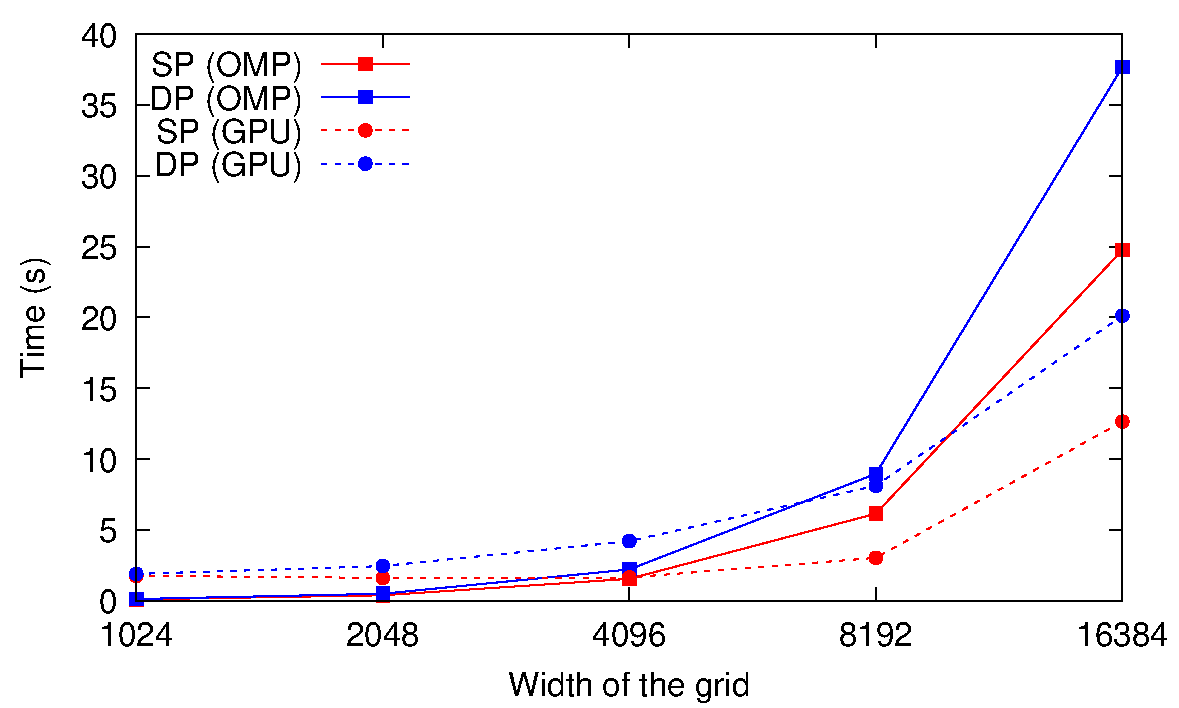
\includegraphics[width=.85\textwidth]{im/result_GPU_Laplace}
		\caption{Results for the first 200 iteration with the size of the grid of the Laplace procedure on a CPU (with \cdx{OMP\_NUM\_THREADS=4}) and a GPU.}
	\end{figure}
	Now that gets interesting! 
\end{frame}